%===================================== CHAP 1 =================================
\chapter{System description}
\section{{Project description}}
The objective of this project is to integrate an NFC Transponder chip into a larger system. Designing a printed circuit board (PCB) containing an NFC chip and an external antenna.
\section{System specifications}
The system specifications are as follows. The NFC chip must have an $I^2C$ interface for communication. Be Compatible with a 2.5 V power rating. Support ISO/IEC 14443 that defines transmission protocols for communicating with contactless integrated circuit cards. 13.56 MHz communication frequency. Support an external antenna. The cost should be kept to a minimum. \\

Having this as a start point, it was concluded that the RF430CL330H chip would be a good choice. A table of specification for this chip is shown in Table \ref{tb:sepc}.


\section{Block Diagram}
The block diagram shows the communication between the NFC Transponder and the host system. Using the Nexus 5X phone as an NFC reader.

\begin{figure}[h]
\begin{center}
\center
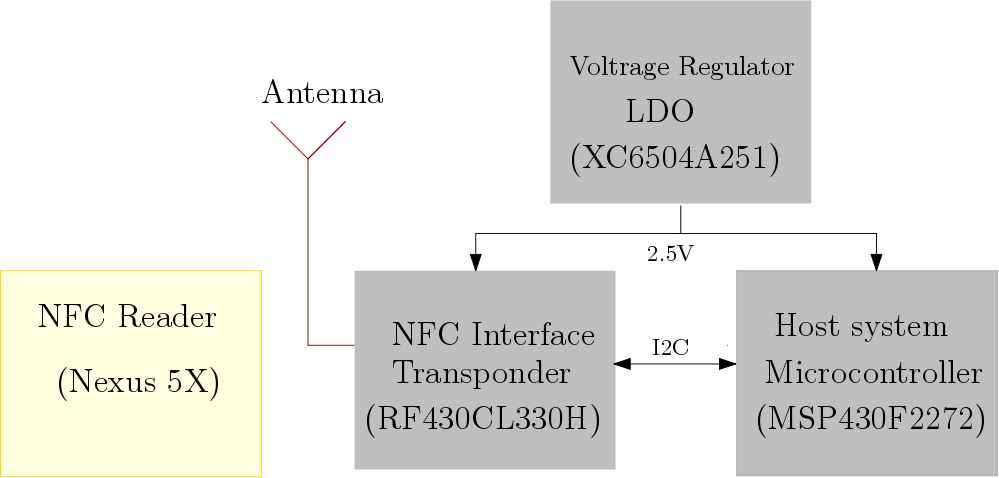
\includegraphics[scale=0.4]{Illustrations/block_diagram.png}  
\caption{System's Block Diagram}
\label{eagle_package}
\end{center}
\end{figure}


%\pagebreak
\section{Introduction to RF430CL330H}


The RF430CL330H NFC Transponder chip offers read/write possibility in NDEF (NFC Data Exchange Format) which is a standard data format maintained by the NFC Forum.  Table \ref{tb:sepc} shows the parameters of interest, taking the specifications in mind.

\begin{figure}[h]
\begin{flushright}
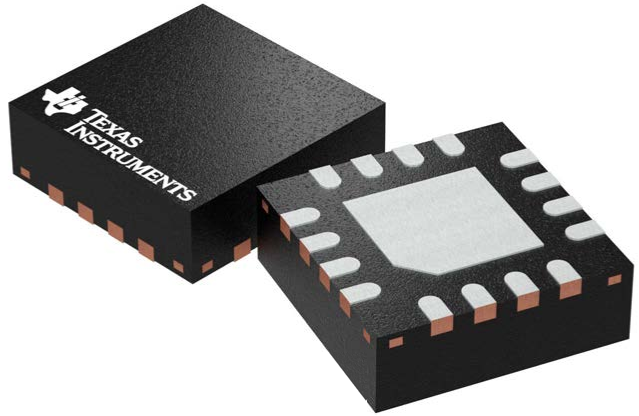
\includegraphics[scale=0.4]{Illustrations/RF430CL330H.png}  
\caption{\texttt{VQFN package from \cite{TexasInstruments2012}}}
\end{flushright}
\end{figure}



\begin{table}[!h]
\centering
\begin{tabular}{|c|c|}
\hline 
\rowcolor{Gray}
Parameter & Specification \\ 
\hline 
Power supply range & 2 V - 3.6 V \\ 
\hline 
Communcation & SPI and $I^2C$ \\ 
\hline 
RF standard support & ISO/IEC 14443B and NFC Tag Type 4B   \\ 
\hline 
Radio Frequency & 13.56 MHz \\ 
\hline 
Antenna connection & Differential \\ 
\hline 
Data rate & 848 kbps \\ 
\hline 
Package size & 9 mm2: 3 x 3(VQFN)    \\ 
\hline 
Unit price &  \$1.53  \\ 
\hline 
\end{tabular} 
\caption{RF430CL330H specifications} \label{tb:sepc} 
\end{table}

